\documentclass[ignorenonframetext,]{beamer}
\setbeamertemplate{caption}[numbered]
\setbeamertemplate{caption label separator}{: }
\setbeamercolor{caption name}{fg=normal text.fg}
\beamertemplatenavigationsymbolsempty
\usepackage{lmodern}
\usepackage{amssymb,amsmath}
\usepackage{ifxetex,ifluatex}
\usepackage{fixltx2e} % provides \textsubscript
\ifnum 0\ifxetex 1\fi\ifluatex 1\fi=0 % if pdftex
  \usepackage[T1]{fontenc}
  \usepackage[utf8]{inputenc}
\else % if luatex or xelatex
  \ifxetex
    \usepackage{mathspec}
  \else
    \usepackage{fontspec}
  \fi
  \defaultfontfeatures{Ligatures=TeX,Scale=MatchLowercase}
\fi
\usetheme[]{Amsterdam}
% use upquote if available, for straight quotes in verbatim environments
\IfFileExists{upquote.sty}{\usepackage{upquote}}{}
% use microtype if available
\IfFileExists{microtype.sty}{%
\usepackage{microtype}
\UseMicrotypeSet[protrusion]{basicmath} % disable protrusion for tt fonts
}{}
\newif\ifbibliography
\hypersetup{
            pdftitle={Introduction to Data Analysis in R},
            pdfauthor={Andrew Proctor},
            pdfborder={0 0 0},
            breaklinks=true}
\urlstyle{same}  % don't use monospace font for urls
\usepackage{color}
\usepackage{fancyvrb}
\newcommand{\VerbBar}{|}
\newcommand{\VERB}{\Verb[commandchars=\\\{\}]}
\DefineVerbatimEnvironment{Highlighting}{Verbatim}{commandchars=\\\{\}}
% Add ',fontsize=\small' for more characters per line
\usepackage{framed}
\definecolor{shadecolor}{RGB}{42,33,28}
\newenvironment{Shaded}{\begin{snugshade}}{\end{snugshade}}
\newcommand{\KeywordTok}[1]{\textcolor[rgb]{0.26,0.66,0.93}{\textbf{#1}}}
\newcommand{\DataTypeTok}[1]{\textcolor[rgb]{0.74,0.68,0.62}{\underline{#1}}}
\newcommand{\DecValTok}[1]{\textcolor[rgb]{0.27,0.67,0.26}{#1}}
\newcommand{\BaseNTok}[1]{\textcolor[rgb]{0.27,0.67,0.26}{#1}}
\newcommand{\FloatTok}[1]{\textcolor[rgb]{0.27,0.67,0.26}{#1}}
\newcommand{\ConstantTok}[1]{\textcolor[rgb]{0.74,0.68,0.62}{#1}}
\newcommand{\CharTok}[1]{\textcolor[rgb]{0.02,0.61,0.04}{#1}}
\newcommand{\SpecialCharTok}[1]{\textcolor[rgb]{0.02,0.61,0.04}{#1}}
\newcommand{\StringTok}[1]{\textcolor[rgb]{0.02,0.61,0.04}{#1}}
\newcommand{\VerbatimStringTok}[1]{\textcolor[rgb]{0.02,0.61,0.04}{#1}}
\newcommand{\SpecialStringTok}[1]{\textcolor[rgb]{0.02,0.61,0.04}{#1}}
\newcommand{\ImportTok}[1]{\textcolor[rgb]{0.74,0.68,0.62}{#1}}
\newcommand{\CommentTok}[1]{\textcolor[rgb]{0.00,0.40,1.00}{\textit{#1}}}
\newcommand{\DocumentationTok}[1]{\textcolor[rgb]{0.00,0.40,1.00}{\textit{#1}}}
\newcommand{\AnnotationTok}[1]{\textcolor[rgb]{0.00,0.40,1.00}{\textbf{\textit{#1}}}}
\newcommand{\CommentVarTok}[1]{\textcolor[rgb]{0.74,0.68,0.62}{#1}}
\newcommand{\OtherTok}[1]{\textcolor[rgb]{0.74,0.68,0.62}{#1}}
\newcommand{\FunctionTok}[1]{\textcolor[rgb]{1.00,0.58,0.35}{\textbf{#1}}}
\newcommand{\VariableTok}[1]{\textcolor[rgb]{0.74,0.68,0.62}{#1}}
\newcommand{\ControlFlowTok}[1]{\textcolor[rgb]{0.26,0.66,0.93}{\textbf{#1}}}
\newcommand{\OperatorTok}[1]{\textcolor[rgb]{0.74,0.68,0.62}{#1}}
\newcommand{\BuiltInTok}[1]{\textcolor[rgb]{0.74,0.68,0.62}{#1}}
\newcommand{\ExtensionTok}[1]{\textcolor[rgb]{0.74,0.68,0.62}{#1}}
\newcommand{\PreprocessorTok}[1]{\textcolor[rgb]{0.74,0.68,0.62}{\textbf{#1}}}
\newcommand{\AttributeTok}[1]{\textcolor[rgb]{0.74,0.68,0.62}{#1}}
\newcommand{\RegionMarkerTok}[1]{\textcolor[rgb]{0.74,0.68,0.62}{#1}}
\newcommand{\InformationTok}[1]{\textcolor[rgb]{0.00,0.40,1.00}{\textbf{\textit{#1}}}}
\newcommand{\WarningTok}[1]{\textcolor[rgb]{1.00,1.00,0.00}{\textbf{#1}}}
\newcommand{\AlertTok}[1]{\textcolor[rgb]{1.00,1.00,0.00}{#1}}
\newcommand{\ErrorTok}[1]{\textcolor[rgb]{1.00,1.00,0.00}{\textbf{#1}}}
\newcommand{\NormalTok}[1]{\textcolor[rgb]{0.74,0.68,0.62}{#1}}
\usepackage{longtable,booktabs}
\usepackage{caption}
% These lines are needed to make table captions work with longtable:
\makeatletter
\def\fnum@table{\tablename~\thetable}
\makeatother
\usepackage{graphicx,grffile}
\makeatletter
\def\maxwidth{\ifdim\Gin@nat@width>\linewidth\linewidth\else\Gin@nat@width\fi}
\def\maxheight{\ifdim\Gin@nat@height>\textheight0.8\textheight\else\Gin@nat@height\fi}
\makeatother
% Scale images if necessary, so that they will not overflow the page
% margins by default, and it is still possible to overwrite the defaults
% using explicit options in \includegraphics[width, height, ...]{}
\setkeys{Gin}{width=\maxwidth,height=\maxheight,keepaspectratio}

% Prevent slide breaks in the middle of a paragraph:
\widowpenalties 1 10000
\raggedbottom

\AtBeginPart{
  \let\insertpartnumber\relax
  \let\partname\relax
  \frame{\partpage}
}
\AtBeginSection{
  \ifbibliography
  \else
    \let\insertsectionnumber\relax
    \let\sectionname\relax
    \frame{\sectionpage}
  \fi
}
\AtBeginSubsection{
  \let\insertsubsectionnumber\relax
  \let\subsectionname\relax
  \frame{\subsectionpage}
}

\setlength{\parindent}{0pt}
\setlength{\parskip}{6pt plus 2pt minus 1pt}
\setlength{\emergencystretch}{3em}  % prevent overfull lines
\providecommand{\tightlist}{%
  \setlength{\itemsep}{0pt}\setlength{\parskip}{0pt}}
\setcounter{secnumdepth}{0}
\usepackage{color}
\usepackage{hyperref}
\definecolor{cornflower}{HTML}{1c86ee}
\hypersetup{ colorlinks=true, linkcolor=cornflower, filecolor=magenta, urlcolor=blue, }

\title{Introduction to Data Analysis in R}
\subtitle{Module 5: Regression analysis and data visualization}
\author{Andrew Proctor}
\institute{\href{mailto:andrew.proctor@phdstudent.hhs.se}{\nolinkurl{andrew.proctor@phdstudent.hhs.se}}}
\date{February 18, 2019}

\begin{document}
\frame{\titlepage}

\begin{frame}
\tableofcontents[hideallsubsections]
\end{frame}

\section{Intro}\label{intro}

\begin{frame}{Goals for today}

\begin{enumerate}
\def\labelenumi{\arabic{enumi}.}
\tightlist
\item
  Introduce basics of linear regression models in R, including model
  diagnostics and specifying error variance structures.
\item
  Introduce further methods for panel data and instrumental variables.
\item
  Explore data visualization methods using the ggplot2 package.
\end{enumerate}

\end{frame}

\section{Regression Basics}\label{regression-basics}

\begin{frame}[fragile]{Linear Regression}

The basic method of performing a linear regression in R is to the use
the
\href{https://www.rdocumentation.org/packages/stats/versions/3.4.3/topics/lm}{lm()}
function.

\begin{itemize}
\tightlist
\item
  To see the parameter estimates alone, you can just call the
  \texttt{lm()} function. But much more results are available if you
  save the results to a regression output object, which can then be
  accessed using the
  \href{https://www.rdocumentation.org/packages/base/versions/3.4.3/topics/summary}{summary()}
  function.
\end{itemize}

Syntax:

\begin{Shaded}
\begin{Highlighting}[]
\NormalTok{myregobject <-}\StringTok{ }\KeywordTok{lm}\NormalTok{(y }\OperatorTok{~}\StringTok{ }\NormalTok{x1 }\OperatorTok{+}\StringTok{ }\NormalTok{x2 }\OperatorTok{+}\StringTok{ }\NormalTok{x3 }\OperatorTok{+}\StringTok{ }\NormalTok{x4, }
                  \DataTypeTok{data =}\NormalTok{ mydataset)}
\end{Highlighting}
\end{Shaded}

\end{frame}

\begin{frame}[fragile]{CEX linear regression example}

\begin{Shaded}
\begin{Highlighting}[]
\KeywordTok{lm}\NormalTok{(expenditures }\OperatorTok{~}\StringTok{ }\NormalTok{educ_ref, }\DataTypeTok{data=}\NormalTok{cex_data)}
\end{Highlighting}
\end{Shaded}

\begin{verbatim}
## 
## Call:
## lm(formula = expenditures ~ educ_ref, data = cex_data)
## 
## Coefficients:
## (Intercept)     educ_ref  
##      -641.1        109.3
\end{verbatim}

\begin{Shaded}
\begin{Highlighting}[]
\NormalTok{cex_linreg <-}\StringTok{ }\KeywordTok{lm}\NormalTok{(expenditures }\OperatorTok{~}\StringTok{ }\NormalTok{educ_ref, }
                 \DataTypeTok{data=}\NormalTok{cex_data)}
\end{Highlighting}
\end{Shaded}

\end{frame}

\begin{frame}[fragile]{CEX linear regression example ctd}

\begin{Shaded}
\begin{Highlighting}[]
\KeywordTok{summary}\NormalTok{(cex_linreg)}
\end{Highlighting}
\end{Shaded}

\begin{verbatim}
## 
## Call:
## lm(formula = expenditures ~ educ_ref, data = cex_data)
## 
## Residuals:
##     Min      1Q  Median      3Q     Max 
## -541109    -899    -690    -506  965001 
## 
## Coefficients:
##             Estimate Std. Error t value Pr(>|t|)    
## (Intercept) -641.062     97.866   -6.55 5.75e-11 ***
## educ_ref     109.350      7.137   15.32  < 2e-16 ***
## ---
## Signif. codes:  0 '***' 0.001 '**' 0.01 '*' 0.05 '.' 0.1 ' ' 1
## 
## Residual standard error: 7024 on 305970 degrees of freedom
##   (75769 observations deleted due to missingness)
## Multiple R-squared:  0.0007666,  Adjusted R-squared:  0.0007634 
## F-statistic: 234.7 on 1 and 305970 DF,  p-value: < 2.2e-16
\end{verbatim}

\end{frame}

\begin{frame}[fragile]{Formatting regression output: tidyr}

With the
\href{https://www.rdocumentation.org/packages/broom/versions/0.4.3/topics/tidy}{tidy()}
function from the
\href{https://www.rdocumentation.org/packages/broom}{broom} package, you
can easily create standard regression output tables.

\begin{Shaded}
\begin{Highlighting}[]
\KeywordTok{library}\NormalTok{(broom)}
\KeywordTok{tidy}\NormalTok{(cex_linreg)}
\end{Highlighting}
\end{Shaded}

\begin{longtable}[]{@{}lrrrr@{}}
\toprule
term & estimate & std.error & statistic & p.value\tabularnewline
\midrule
\endhead
(Intercept) & -641.0622 & 97.866411 & -6.550381 & 0\tabularnewline
educ\_ref & 109.3498 & 7.137046 & 15.321432 & 0\tabularnewline
\bottomrule
\end{longtable}

\end{frame}

\begin{frame}[fragile]{Formatting regression output: stargazer}

Another really good option for creating compelling regression and
summary output tables is the
\href{https://www.rdocumentation.org/packages/stargazer/}{stargazer}
package.

\begin{itemize}
\tightlist
\item
  If you write your reports in LaTex, it's especially useful.
\end{itemize}

\begin{Shaded}
\begin{Highlighting}[]
\CommentTok{# From console:  install.packages("stargazer")}

\KeywordTok{library}\NormalTok{(stargazer)}

\KeywordTok{stargazer}\NormalTok{(cex_linreg, }\DataTypeTok{header=}\OtherTok{FALSE}\NormalTok{, }\DataTypeTok{type=}\StringTok{'latex'}\NormalTok{)}
\end{Highlighting}
\end{Shaded}

\end{frame}

\begin{frame}{Stargazer output}

\begin{table}[!htbp] \centering 
  \caption{} 
  \label{} 
\begin{tabular}{@{\extracolsep{5pt}}lc} 
\\[-1.8ex]\hline 
\hline \\[-1.8ex] 
 & \multicolumn{1}{c}{\textit{Dependent variable:}} \\ 
\cline{2-2} 
\\[-1.8ex] & expenditures \\ 
\hline \\[-1.8ex] 
 educ\_ref & 109.350$^{***}$ \\ 
  & (7.137) \\ 
  Constant & $-$641.062$^{***}$ \\ 
  & (97.866) \\ 
 \hline \\[-1.8ex] 
Observations & 305,972 \\ 
R$^{2}$ & 0.001 \\ 
Adjusted R$^{2}$ & 0.001 \\ 
Residual Std. Error & 7,024.151 (df = 305970) \\ 
F Statistic & 234.746$^{***}$ (df = 1; 305970) \\ 
\hline 
\hline \\[-1.8ex] 
\textit{Note:}  & \multicolumn{1}{r}{$^{*}$p$<$0.1; $^{**}$p$<$0.05; $^{***}$p$<$0.01} \\ 
\end{tabular} 
\end{table}

\end{frame}

\begin{frame}[fragile]{Interactions and indicator variables}

Including interaction terms and indicator variables in R is very easy.

\begin{itemize}
\item
  Including any variables coded as factors (ie categorical variables)
  will automatically include indicators for each value of the factor.
\item
  To specify interaction terms, just specify \texttt{varX1*varX2}.
\item
  To specify higher order terms, write it mathematically inside of
  \textbf{I()}.
\end{itemize}

\textbf{Example:}

\begin{Shaded}
\begin{Highlighting}[]
\NormalTok{wages_reg <-}\StringTok{ }\KeywordTok{lm}\NormalTok{(wage }\OperatorTok{~}\StringTok{ }\NormalTok{schooling }\OperatorTok{+}\StringTok{ }\NormalTok{sex }\OperatorTok{+}\StringTok{ }
\StringTok{          }\NormalTok{schooling}\OperatorTok{*}\NormalTok{sex }\OperatorTok{+}\StringTok{ }\KeywordTok{I}\NormalTok{(exper}\OperatorTok{^}\DecValTok{2}\NormalTok{), }\DataTypeTok{data=}\NormalTok{wages)}
\end{Highlighting}
\end{Shaded}

\end{frame}

\begin{frame}[fragile]{Example with interactions and factors}

\begin{Shaded}
\begin{Highlighting}[]
\KeywordTok{tidy}\NormalTok{(wages_reg)}
\end{Highlighting}
\end{Shaded}

\begin{longtable}[]{@{}lrrrr@{}}
\toprule
term & estimate & std.error & statistic & p.value\tabularnewline
\midrule
\endhead
(Intercept) & -2.0530687 & 0.6110201 & -3.3600672 &
0.0007881\tabularnewline
schooling & 0.5672762 & 0.0500783 & 11.3277746 &
0.0000000\tabularnewline
sexmale & -0.3256979 & 0.7790055 & -0.4180945 & 0.6759053\tabularnewline
I(exper\^{}2) & 0.0075173 & 0.0014436 & 5.2072237 &
0.0000002\tabularnewline
schooling:sexmale & 0.1431400 & 0.0659669 & 2.1698748 &
0.0300877\tabularnewline
\bottomrule
\end{longtable}

\end{frame}

\begin{frame}[fragile]{Setting reference groups for factors}

By default, when including factors in R regression, the first
\emph{level} of the factor is treated as the omitted reference group.

\begin{itemize}
\tightlist
\item
  An easy way to instead specify the omitted reference group is to use
  the
  \href{https://www.rdocumentation.org/packages/stats/versions/3.4.3/topics/relevel}{relevel()}
  function.
\end{itemize}

\textbf{Example:}

\begin{Shaded}
\begin{Highlighting}[]
\NormalTok{wages}\OperatorTok{$}\NormalTok{sex <-}\StringTok{ }\NormalTok{wages}\OperatorTok{$}\NormalTok{sex }\OperatorTok\StringTok{ }\KeywordTok{relevel}\NormalTok{(}\DataTypeTok{ref=}\StringTok{"male"}\NormalTok{)}
\NormalTok{wagereg2 <-}\StringTok{ }\KeywordTok{lm}\NormalTok{(wage }\OperatorTok{~}\StringTok{ }\NormalTok{sex, }\DataTypeTok{data=}\NormalTok{wages); }\KeywordTok{tidy}\NormalTok{(wagereg2)}
\end{Highlighting}
\end{Shaded}

\begin{longtable}[]{@{}lrrrr@{}}
\toprule
term & estimate & std.error & statistic & p.value\tabularnewline
\midrule
\endhead
(Intercept) & 6.313021 & 0.0774650 & 81.49511 & 0\tabularnewline
sexfemale & -1.166097 & 0.1122422 & -10.38912 & 0\tabularnewline
\bottomrule
\end{longtable}

\end{frame}

\begin{frame}[fragile]{Useful output from regression}

A couple of useful data elements that are created with a regression
output object are fitted values and residuals. You can easily access
them as follows:

\begin{itemize}
\tightlist
\item
  \textbf{Residuals:} Use the
  \href{https://www.rdocumentation.org/packages/stats/versions/3.4.3/topics/residuals}{residuals()}
  function.
\end{itemize}

\begin{Shaded}
\begin{Highlighting}[]
\NormalTok{myresiduals <-}\StringTok{ }\KeywordTok{residuals}\NormalTok{(myreg)}
\end{Highlighting}
\end{Shaded}

\begin{itemize}
\tightlist
\item
  \textbf{Predicted values:} Use the
  \href{https://www.rdocumentation.org/packages/stats/versions/3.4.3/topics/fitted}{fitted()}
  function.
\end{itemize}

\begin{Shaded}
\begin{Highlighting}[]
\NormalTok{myfittedvalues <-}\StringTok{ }\KeywordTok{fitted}\NormalTok{(myreg)}
\end{Highlighting}
\end{Shaded}

\end{frame}

\section{Model Testing}\label{model-testing}

\begin{frame}[fragile]{Using the lmtest package}

The main package for specification testing of linear regressions in R is
the \href{https://www.rdocumentation.org/packages/lmtest/}{lmtest}
package.

With it, you can:

\begin{itemize}
\tightlist
\item
  test for heteroskedasticity
\item
  test for autocorrelation
\item
  test functional form (eg Ramsey RESET test)
\item
  discriminate between non-nested models and more
\end{itemize}

All of the tests covered here are from the
\href{https://www.rdocumentation.org/packages/lmtest/}{lmtest} package.
As usual, you need to install and initialize the package:

\begin{Shaded}
\begin{Highlighting}[]
\NormalTok{## In the console:  install.packages("lmtest")}
\KeywordTok{library}\NormalTok{(lmtest)}
\end{Highlighting}
\end{Shaded}

\end{frame}

\begin{frame}[fragile]{Testing for heteroskedasticity}

Testing for heteroskedasticity in R can be done with the
\href{https://www.rdocumentation.org/packages/lmtest/versions/0.9-35/topics/bptest}{bptest()}
function from the
\href{https://www.rdocumentation.org/packages/lmtest}{lmtest} to the
model object.

\begin{itemize}
\tightlist
\item
  By default, using a regression object as an argument to
  \href{https://www.rdocumentation.org/packages/lmtest/versions/0.9-35/topics/bptest}{bptest()}
  will perform the Koenker-Bassett version of the Breusch-Pagan test
  (aka `generalized' or `studentized' Breusch-Pagan Test):
\end{itemize}

\begin{Shaded}
\begin{Highlighting}[]
\KeywordTok{bptest}\NormalTok{(wages_reg)}
\end{Highlighting}
\end{Shaded}

\begin{verbatim}
## 
##  studentized Breusch-Pagan test
## 
## data:  wages_reg
## BP = 22.974, df = 4, p-value = 0.0001282
\end{verbatim}

\end{frame}

\begin{frame}[fragile]{Testing for heteroskedasticity ctd}

\begin{itemize}
\tightlist
\item
  If you want the ``standard'' form of the Breusch-Pagan Test, just use:
\end{itemize}

\begin{Shaded}
\begin{Highlighting}[]
\KeywordTok{bptest}\NormalTok{(myreg, }\DataTypeTok{studentize =} \OtherTok{FALSE}\NormalTok{)}
\end{Highlighting}
\end{Shaded}

\begin{itemize}
\item
  You can also perform the White Test of Heteroskedasticity using
  \href{https://www.rdocumentation.org/packages/lmtest/versions/0.9-35/topics/bptest}{bptest()}
  by manually specifying the regressors of the auxiliary regression
  inside of \texttt{bptest}:

  \begin{itemize}
  \tightlist
  \item
    That is, specify the distinct regressors from the main equation,
    their squares, and cross-products.
  \end{itemize}
\end{itemize}

\begin{Shaded}
\begin{Highlighting}[]
\KeywordTok{bptest}\NormalTok{(myreg, }\OperatorTok{~}\StringTok{ }\NormalTok{x1 }\OperatorTok{+}\StringTok{ }\NormalTok{x2 }\OperatorTok{+}\StringTok{ }\NormalTok{x1}\OperatorTok{*}\NormalTok{x2 }\OperatorTok{+}\StringTok{ }\KeywordTok{I}\NormalTok{(x1}\OperatorTok{^}\DecValTok{2}\NormalTok{) }\OperatorTok{+}\StringTok{ }
\StringTok{         }\KeywordTok{I}\NormalTok{(x2}\OperatorTok{^}\DecValTok{2}\NormalTok{), }\DataTypeTok{data=}\NormalTok{mydata)}
\end{Highlighting}
\end{Shaded}

\end{frame}

\begin{frame}[fragile]{Functional form}

The \textbf{Ramsey RESET Test} tests functional form by evaluating if
higher order terms have any explanatory value.

\begin{Shaded}
\begin{Highlighting}[]
\KeywordTok{resettest}\NormalTok{(wages_reg)}
\end{Highlighting}
\end{Shaded}

\begin{verbatim}
## 
##  RESET test
## 
## data:  wages_reg
## RESET = 7.1486, df1 = 2, df2 = 3287, p-value = 0.0007983
\end{verbatim}

\end{frame}

\begin{frame}[fragile]{Testing for autocorrelation: Breusch-Godfrey
test}

\begin{Shaded}
\begin{Highlighting}[]
\KeywordTok{bgtest}\NormalTok{(wages_reg)}
\end{Highlighting}
\end{Shaded}

\begin{verbatim}
## 
##  Breusch-Godfrey test for serial correlation of order up to 1
## 
## data:  wages_reg
## LM test = 7.0938, df = 1, p-value = 0.007735
\end{verbatim}

\end{frame}

\begin{frame}[fragile]{Testing for autocorrelation: Durbin-Watson test}

\begin{Shaded}
\begin{Highlighting}[]
\KeywordTok{dwtest}\NormalTok{(wages_reg)}
\end{Highlighting}
\end{Shaded}

\begin{verbatim}
## 
##  Durbin-Watson test
## 
## data:  wages_reg
## DW = 1.9073, p-value = 0.003489
## alternative hypothesis: true autocorrelation is greater than 0
\end{verbatim}

\end{frame}

\begin{frame}{Specifying the variance structure}

In practice, errors should \emph{almost always} be specified in a manner
that is heteroskedasticity and autocorrelation consistent.

\begin{itemize}
\item
  In Stata, you can pretty much always use the \textbf{robust} option.
\item
  In R, you should more explicitly specify the variance structure.

  \begin{itemize}
  \item
    The
    \href{https://cran.r-project.org/web/packages/sandwich/}{sandwich}
    allows for specification of heteroskedasticity-robust,
    cluster-robust, and heteroskedasticity and autocorrelation-robust
    error structures.
  \item
    These can then be used with t-tests
    {[}\href{https://www.rdocumentation.org/packages/lmtest/versions/0.9-35/topics/coeftest}{coeftest()}{]}
    and F-tests
    {[}\href{https://www.rdocumentation.org/packages/lmtest/versions/0.9-35/topics/waldtest}{waldtest()}{]}
    from \href{https://www.rdocumentation.org/packages/lmtest}{lmtest}.
  \end{itemize}
\end{itemize}

\end{frame}

\begin{frame}{Heteroskedasticity-robust errors}

\(HC_1\) Errors (MacKinnon and White, 1985):
\(\Sigma = \frac{n}{n-k}diag{\hat\{u_i}^2\}\)

\begin{itemize}
\tightlist
\item
  Default heteroskedasticity-robust errors used by Stata with
  \textbf{robust}
\end{itemize}

\(HC_3\) Errors (Davidson and MacKinnon, 1993):
\(\Sigma = diag \{ \big( \frac{\hat{u_i}}{1-h_i} \big)^2 \}\)

\begin{itemize}
\item
  Approximation of the jackknife covariance estimator
\item
  Recommended in some studies over \(HC_1\) because it is better at
  keeping nominal size with only a small loss of power in the presence
  of heteroskedasticity.
\end{itemize}

\end{frame}

\begin{frame}[fragile]{Heteroskedasticity-robust errors example}

\begin{Shaded}
\begin{Highlighting}[]
\NormalTok{cex_reg <-}\StringTok{ }\KeywordTok{lm}\NormalTok{(expenditures }\OperatorTok{~}\StringTok{ }\NormalTok{hh_size }\OperatorTok{+}\StringTok{ }\NormalTok{educ_ref }\OperatorTok{+}\StringTok{ }
\StringTok{                }\NormalTok{region, }\DataTypeTok{data=}\NormalTok{cex_data)}
\KeywordTok{tidy}\NormalTok{(}\KeywordTok{coeftest}\NormalTok{(cex_reg, }\DataTypeTok{vcov =} 
                \KeywordTok{vcovHC}\NormalTok{(cex_reg, }\DataTypeTok{type=}\StringTok{"HC1"}\NormalTok{)))}
\end{Highlighting}
\end{Shaded}

\begin{longtable}[]{@{}lrrrr@{}}
\toprule
term & estimate & std.error & statistic & p.value\tabularnewline
\midrule
\endhead
(Intercept) & -553.26201 & 94.106216 & -5.879123 & 0e+00\tabularnewline
hh\_size & -298.33622 & 14.262224 & -20.917932 & 0e+00\tabularnewline
educ\_ref & 109.46626 & 7.190421 & 15.223901 & 0e+00\tabularnewline
region & 83.15485 & 15.274695 & 5.443962 & 1e-07\tabularnewline
\bottomrule
\end{longtable}

\end{frame}

\begin{frame}[fragile]{Computing marginal effects}

In linear regressions where the regressors and regressors are in
``levels'', the coefficients are of course equal to the marginal
effects.

\begin{itemize}
\item
  But if the regression is nonlinear or a regressor enter in e.g.~in
  logs or quadratics, then marginal effects may be more important than
  coefficients.
\item
  You can use the package
  \href{https://www.rdocumentation.org/packages/margins/versions/0.3.0}{margins}
  to get marginal effects.
\end{itemize}

\begin{Shaded}
\begin{Highlighting}[]
\CommentTok{# install.packages("margins")}
\KeywordTok{library}\NormalTok{(margins)}
\end{Highlighting}
\end{Shaded}

\end{frame}

\begin{frame}[fragile]{Marginal effects example}

We can get the Average Marginal Effects by using \texttt{summary} with
\textbf{margins}:

\begin{Shaded}
\begin{Highlighting}[]
\KeywordTok{summary}\NormalTok{(}\KeywordTok{margins}\NormalTok{(wages_reg))}
\end{Highlighting}
\end{Shaded}

\begin{longtable}[]{@{}lrrrrrr@{}}
\toprule
factor & AME & SE & z & p & lower & upper\tabularnewline
\midrule
\endhead
exper & 0.1209297 & 0.0232234 & 5.207226 & 2e-07 & 0.0754126 &
0.1664468\tabularnewline
schooling & 0.6422357 & 0.0334052 & 19.225648 & 0e+00 & 0.5767628 &
0.7077086\tabularnewline
sexfemale & -1.3390973 & 0.1077331 & -12.429771 & 0e+00 & -1.5502502 &
-1.1279444\tabularnewline
\bottomrule
\end{longtable}

\end{frame}

\section{Further regression methods}\label{further-regression-methods}

\begin{frame}[fragile]{Panel regression: first differences}

The package \href{https://www.rdocumentation.org/packages/plm}{plm}
provides a wide variety of estimation methods and diagnostics for panel
data.

\begin{itemize}
\item
  We will cover two common panel data estimators, first-differences
  regression and fixed effects regression.
\item
  To estimate first-differences estimator, use the
  \href{https://www.rdocumentation.org/packages/plm/versions/1.6-5/topics/plm}{plm()}
  in the plm package.
\end{itemize}

\begin{Shaded}
\begin{Highlighting}[]
\KeywordTok{library}\NormalTok{(plm)}
\end{Highlighting}
\end{Shaded}

\textbf{Syntax:}

\begin{Shaded}
\begin{Highlighting}[]
\NormalTok{myreg <-}\StringTok{ }\KeywordTok{plm}\NormalTok{(y }\OperatorTok{~}\StringTok{ }\NormalTok{x1 }\OperatorTok{+}\StringTok{ }\NormalTok{x2 }\OperatorTok{+}\StringTok{ }\NormalTok{x3, }\DataTypeTok{data =}\NormalTok{ mydata, }
          \DataTypeTok{index=}\KeywordTok{c}\NormalTok{(}\StringTok{"groupvar"}\NormalTok{, }\StringTok{"timevar"}\NormalTok{), }\DataTypeTok{model=}\StringTok{"fd"}\NormalTok{)}
\end{Highlighting}
\end{Shaded}

\end{frame}

\begin{frame}[fragile]{Panel regression: fixed effects}

Of course, in most cases fixed effects regression is a more efficient
alternative to first-difference regression.

To use fixed effects regression, instead specify the argument
\textbf{model = ``within''}.

\begin{itemize}
\tightlist
\item
  Use the option \textbf{effect = ``twoway''} to include group and year
  fixed effects.
\end{itemize}

\begin{Shaded}
\begin{Highlighting}[]
\NormalTok{myreg <-}\StringTok{ }\KeywordTok{plm}\NormalTok{(y }\OperatorTok{~}\StringTok{ }\NormalTok{x1 }\OperatorTok{+}\StringTok{ }\NormalTok{x2 }\OperatorTok{+}\StringTok{ }\NormalTok{x3, }\DataTypeTok{data =}\NormalTok{ mydata, }
             \DataTypeTok{index=}\KeywordTok{c}\NormalTok{(}\StringTok{"groupvar"}\NormalTok{, }\StringTok{"timevar"}\NormalTok{), }
             \DataTypeTok{model=}\StringTok{"within"}\NormalTok{, }\DataTypeTok{effect =} \StringTok{"twoway"}\NormalTok{)}
\end{Highlighting}
\end{Shaded}

\end{frame}

\begin{frame}[fragile]{A crime example}

\begin{Shaded}
\begin{Highlighting}[]
\NormalTok{crime_NC <-}\StringTok{ }\NormalTok{Crime }\OperatorTok\StringTok{ }\KeywordTok{as.tibble}\NormalTok{() }\OperatorTok\StringTok{ }
\StringTok{  }\KeywordTok{select}\NormalTok{(county, year, crmrte, polpc, region, smsa, }
\NormalTok{  taxpc) }\OperatorTok\StringTok{ }\KeywordTok{rename}\NormalTok{(}\DataTypeTok{crimerate=}\NormalTok{crmrte, }
  \DataTypeTok{police_pc =}\NormalTok{ polpc, }\DataTypeTok{urban=}\NormalTok{smsa, }\DataTypeTok{tax_pc=}\NormalTok{taxpc)}
\NormalTok{crime_NC[}\DecValTok{1}\OperatorTok{:}\DecValTok{2}\NormalTok{,]}
\end{Highlighting}
\end{Shaded}

\begin{longtable}[]{@{}rrrrllr@{}}
\toprule
county & year & crimerate & police\_pc & region & urban &
tax\_pc\tabularnewline
\midrule
\endhead
1 & 81 & 0.0398849 & 0.0017868 & central & no & 25.69763\tabularnewline
1 & 82 & 0.0383449 & 0.0017666 & central & no & 24.87425\tabularnewline
\bottomrule
\end{longtable}

\end{frame}

\begin{frame}[fragile]{First differences regression on the crime
dataset}

\begin{Shaded}
\begin{Highlighting}[]
\NormalTok{crime_reg <-}\StringTok{ }\KeywordTok{plm}\NormalTok{(crimerate }\OperatorTok{~}\StringTok{ }\NormalTok{police_pc }\OperatorTok{+}\StringTok{ }\NormalTok{tax_pc }\OperatorTok{+}
\StringTok{                }\NormalTok{region }\OperatorTok{+}\StringTok{ }\NormalTok{urban, }\DataTypeTok{data=}\NormalTok{crime_NC, }
                \DataTypeTok{index=}\KeywordTok{c}\NormalTok{(}\StringTok{"county"}\NormalTok{, }\StringTok{"year"}\NormalTok{), }\DataTypeTok{model=}\StringTok{"fd"}\NormalTok{)}
\KeywordTok{tidy}\NormalTok{(crime_reg)}
\end{Highlighting}
\end{Shaded}

\begin{longtable}[]{@{}lrrrr@{}}
\toprule
term & estimate & std.error & statistic & p.value\tabularnewline
\midrule
\endhead
(Intercept) & 0.0001289 & 0.0003738 & 0.3448421 &
0.7303481\tabularnewline
police\_pc & 2.0610223 & 0.1997587 & 10.3175609 &
0.0000000\tabularnewline
tax\_pc & 0.0000011 & 0.0000515 & 0.0209585 & 0.9832866\tabularnewline
\bottomrule
\end{longtable}

\end{frame}

\begin{frame}[fragile]{Fixed effects regression on the crime dataset}

\begin{Shaded}
\begin{Highlighting}[]
\NormalTok{crime_reg <-}\StringTok{ }\KeywordTok{plm}\NormalTok{(crimerate }\OperatorTok{~}\StringTok{ }\NormalTok{police_pc }\OperatorTok{+}\StringTok{ }
\StringTok{                }\NormalTok{tax_pc }\OperatorTok{+}\StringTok{ }\NormalTok{urban, }\DataTypeTok{data=}\NormalTok{crime_NC, }
                \DataTypeTok{index=}\KeywordTok{c}\NormalTok{(}\StringTok{"county"}\NormalTok{, }\StringTok{"year"}\NormalTok{), }
                \DataTypeTok{model=}\StringTok{"within"}\NormalTok{, }\DataTypeTok{effect=}\StringTok{"twoway"}\NormalTok{)}
\KeywordTok{tidy}\NormalTok{(crime_reg)}
\end{Highlighting}
\end{Shaded}

\begin{longtable}[]{@{}lrrrr@{}}
\toprule
term & estimate & std.error & statistic & p.value\tabularnewline
\midrule
\endhead
police\_pc & 1.7782245 & 0.1437963 & 12.366272 &
0.0000000\tabularnewline
tax\_pc & 0.0000627 & 0.0000450 & 1.391503 & 0.1646546\tabularnewline
\bottomrule
\end{longtable}

\end{frame}

\begin{frame}[fragile]{Instrumental variables regression}

The most popular function for doing IV regression is the
\href{https://www.rdocumentation.org/packages/AER/versions/1.2-5/topics/ivreg}{ivreg()}
in the \href{https://www.rdocumentation.org/packages/AER}{AER package}.

\begin{Shaded}
\begin{Highlighting}[]
\KeywordTok{library}\NormalTok{(AER)}
\end{Highlighting}
\end{Shaded}

\textbf{Syntax:}

\begin{Shaded}
\begin{Highlighting}[]
\NormalTok{myivreg <-}\StringTok{ }\KeywordTok{ivreg}\NormalTok{(y }\OperatorTok{~}\StringTok{ }\NormalTok{x1 }\OperatorTok{+}\StringTok{ }\NormalTok{x2 }\OperatorTok{|}\StringTok{ }\NormalTok{z1 }\OperatorTok{+}\StringTok{ }\NormalTok{z2 }\OperatorTok{+}\StringTok{ }\NormalTok{z3, }
                 \DataTypeTok{data =}\NormalTok{ mydata)}
\end{Highlighting}
\end{Shaded}

\end{frame}

\begin{frame}{IV diagnostics}

Three common diagnostic tests are available with the \textbf{summary}
output for regression objects from
\href{https://www.rdocumentation.org/packages/AER/versions/1.2-5/topics/ivreg}{ivreg()}.

\begin{itemize}
\item
  \textbf{Durbin-Wu-Hausman Test of Endogeneity:} Tests for endogeneity
  of suspected endogenous regressor under assumption that instruments
  are exogenous.
\item
  \textbf{F-Test of Weak Instruments}: Typical rule-of-thumb value of 10
  to avoid weak instruments, although you can compare again Stock and
  Yogo (2005) critical values for more precise guidance concerning
  statistical size and relative bias.
\item
  \textbf{Sargan-Hansen Test of Overidentifying Restrictions:} In
  overidentified case, tests if some instruments are endogenous ~~~under
  the initial assumption that all instruments are exogenous.
\end{itemize}

\end{frame}

\begin{frame}[fragile]{IV regression example}

Let's look at an IV regression from the seminal paper ``The Colonial
Origins of Comparative Development'' by Acemogulu, Johnson, and Robinson
(AER 2001)

\begin{Shaded}
\begin{Highlighting}[]
\NormalTok{col_origins <-}\StringTok{ }\KeywordTok{import}\NormalTok{(}\StringTok{"maketable5.dta"}\NormalTok{) }\OperatorTok\StringTok{ }
\StringTok{  }\KeywordTok{as.tibble}\NormalTok{() }\OperatorTok\StringTok{ }\KeywordTok{filter}\NormalTok{(baseco}\OperatorTok{==}\DecValTok{1}\NormalTok{) }\OperatorTok\StringTok{ }
\StringTok{  }\KeywordTok{select}\NormalTok{(logpgp95, avexpr, logem4, shortnam) }\OperatorTok
\StringTok{  }\KeywordTok{rename}\NormalTok{(}\DataTypeTok{logGDP95 =}\NormalTok{ logpgp95, }\DataTypeTok{country =}\NormalTok{ shortnam,}
    \DataTypeTok{legalprotect =}\NormalTok{ avexpr, }\DataTypeTok{log.settler.mort =}\NormalTok{ logem4)}

\NormalTok{col_origins_iv <-}\StringTok{ }\KeywordTok{ivreg}\NormalTok{(logGDP95 }\OperatorTok{~}\StringTok{ }\NormalTok{legalprotect }\OperatorTok{|}\StringTok{ }
\StringTok{      }\NormalTok{log.settler.mort, }\DataTypeTok{data =}\NormalTok{ col_origins)}
\end{Highlighting}
\end{Shaded}

\end{frame}

\begin{frame}[fragile]{IV regression example: estimates}

\begin{Shaded}
\begin{Highlighting}[]
\NormalTok{IVsummary <-}\StringTok{ }\KeywordTok{summary}\NormalTok{(col_origins_iv, }\DataTypeTok{diagnostics =} \OtherTok{TRUE}\NormalTok{)}
\NormalTok{IVsummary[}\StringTok{"coefficients"}\NormalTok{]}
\end{Highlighting}
\end{Shaded}

\begin{verbatim}
## $coefficients
##               Estimate Std. Error  t value     Pr(>|t|)
## (Intercept)  1.9096665  1.0267273 1.859955 6.763720e-02
## legalprotect 0.9442794  0.1565255 6.032753 9.798645e-08
\end{verbatim}

\end{frame}

\begin{frame}[fragile]{IV regression example: diagnostics}

\begin{Shaded}
\begin{Highlighting}[]
\NormalTok{IVsummary[}\StringTok{"diagnostics"}\NormalTok{]}
\end{Highlighting}
\end{Shaded}

\begin{verbatim}
## $diagnostics
##                  df1 df2 statistic      p-value
## Weak instruments   1  62  22.94680 1.076546e-05
## Wu-Hausman         1  61  24.21962 6.852437e-06
## Sargan             0  NA        NA           NA
\end{verbatim}

\end{frame}

\begin{frame}{Further regression methods}

Some useful functions for nonlinear regression include:

\begin{itemize}
\item
  \textbf{Quantile Regression:}
  \href{https://www.rdocumentation.org/packages/quantreg/versions/5.34/topics/rq}{rq()}
  in the
  \href{https://www.rdocumentation.org/packages/quantreg/}{quantreg}
  package.
\item
  \textbf{Limited Dependent Variable Models:}

  \begin{itemize}
  \item
    These models, such as logit and probit (binary choice), or Poisson
    (count model) are incorporated in R as specific cases of a
    \emph{generalized linear model} (GLM).
  \item
    GLM models are estimated in R using the
    \href{https://www.rdocumentation.org/packages/stats/versions/3.4.3/topics/glm}{glm()}
    function in base R.
  \end{itemize}
\item
  \textbf{Regression Discontinutiy:}

  \begin{itemize}
  \tightlist
  \item
    RDD designs can easily be performed in R through a few different
    packages.
  \item
    I suggest using the function
    \href{https://www.rdocumentation.org/packages/rdrobust/versions/0.98/topics/rdrobust}{rdrobust()}
    from the package of ~~~the same name.
  \end{itemize}
\end{itemize}

\end{frame}

\section{Graphs in R}\label{graphs-in-r}

\begin{frame}{Data visualization overview}

One of the strong points of R is creating very high-quality data
visualization.

\begin{itemize}
\item
  R is very good at both ``static'' data visualization and interactive
  data visualization designed for web use.
\item
  Today, I will be covering static data visualization, but here are a
  couple of good resources for interactive visualization:
  {[}\href{http://www.rebeccabarter.com/blog/2017-04-20-interactive/}{1}{]},
  {[}\href{https://www.r-graph-gallery.com/get-the-best-from-ggplotly/}{2}{]}
\end{itemize}

\end{frame}

\begin{frame}[fragile]{ggplot2 for data visualization}

The main package for publication-quality static data visualization in R
is \href{https://www.rdocumentation.org/packages/ggplot2}{ggplot2},
which is part of the tidyverse collection of packages.

\begin{itemize}
\item
  The workhorse function of ggplot2 is
  \href{https://www.rdocumentation.org/packages/ggplot2/versions/2.2.1/topics/ggplot}{ggplot()},
  response for creating a very wide variety of graphs.
\item
  The ``gg'' stands for ``grammar of graphics''. In each
  \href{https://www.rdocumentation.org/packages/ggplot2/versions/2.2.1/topics/ggplot}{ggplot()}
  call, the appearance of the graph is determined by specifying:

  \begin{itemize}
  \tightlist
  \item
    The \textbf{data}(frame) to be used.
  \item
    The \textbf{aes}(thetics) of the graph --- like size, color, x and y
    variables.
  \item
    The \textbf{geom}(etry) of the graph --- type of data to be used.
  \end{itemize}
\end{itemize}

\begin{Shaded}
\begin{Highlighting}[]
\NormalTok{mygraph <-}\StringTok{ }\KeywordTok{ggplot}\NormalTok{(mydata, }\KeywordTok{aes}\NormalTok{(...)) }\OperatorTok{+}\StringTok{ }\KeywordTok{geom}\NormalTok{(...) }\OperatorTok{+}\StringTok{ }\NormalTok{... }
\end{Highlighting}
\end{Shaded}

\end{frame}

\begin{frame}[fragile]{Scatterplots}

First, let's look at a simple scatterplot, which is defined by using the
geometry \textbf{geom\_point()}.

\begin{Shaded}
\begin{Highlighting}[]
\KeywordTok{ggplot}\NormalTok{(col_origins, }\KeywordTok{aes}\NormalTok{(}\DataTypeTok{x=}\NormalTok{legalprotect, }
            \DataTypeTok{y =}\NormalTok{ logGDP95)) }\OperatorTok{+}\StringTok{ }\KeywordTok{geom_point}\NormalTok{() }
\end{Highlighting}
\end{Shaded}

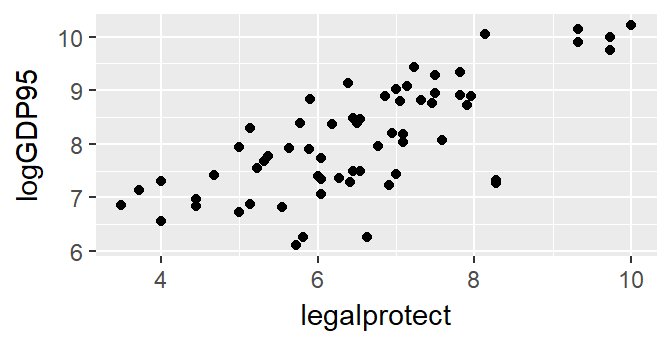
\includegraphics{module5_files/figure-beamer/unnamed-chunk-39-1.pdf}

\end{frame}

\begin{frame}[fragile]{Adding an aesthetic option to the points}

Graphs can be extensively customized using additional arguments inside
of elements:

\begin{Shaded}
\begin{Highlighting}[]
\KeywordTok{ggplot}\NormalTok{(col_origins, }\KeywordTok{aes}\NormalTok{(}\DataTypeTok{x=}\NormalTok{legalprotect,}\DataTypeTok{y =}\NormalTok{ logGDP95)) }\OperatorTok{+}\StringTok{ }
\StringTok{  }\KeywordTok{geom_point}\NormalTok{(}\KeywordTok{aes}\NormalTok{(}\DataTypeTok{size=}\NormalTok{logGDP95))}
\end{Highlighting}
\end{Shaded}

\end{frame}

\begin{frame}{Adding an aesthetic option to the points}

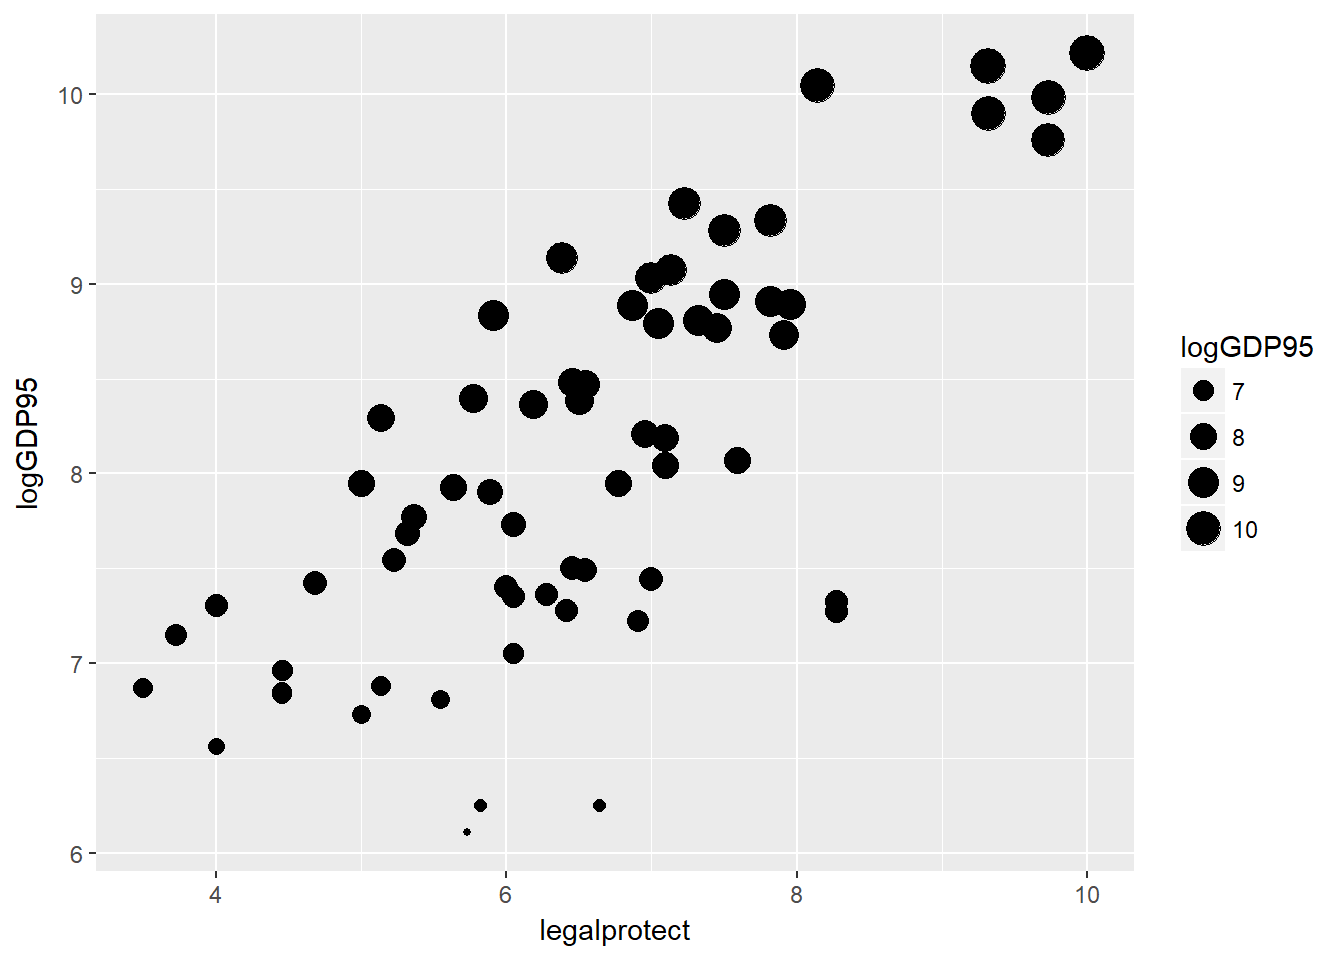
\includegraphics{module5_files/figure-beamer/unnamed-chunk-41-1.pdf}

\end{frame}

\begin{frame}[fragile]{Using country names instead of points}

Instead of using a scatter plot, we could use the names of the data
points in place of the dots.

\begin{Shaded}
\begin{Highlighting}[]
\KeywordTok{ggplot}\NormalTok{(col_origins, }
       \KeywordTok{aes}\NormalTok{(}\DataTypeTok{x=}\NormalTok{legalprotect, }\DataTypeTok{y =}\NormalTok{ logGDP95, }
       \DataTypeTok{label=}\NormalTok{country)) }\OperatorTok{+}\StringTok{  }\KeywordTok{geom_text}\NormalTok{()}
\end{Highlighting}
\end{Shaded}

\end{frame}

\begin{frame}{Using country names instead of points ctd}

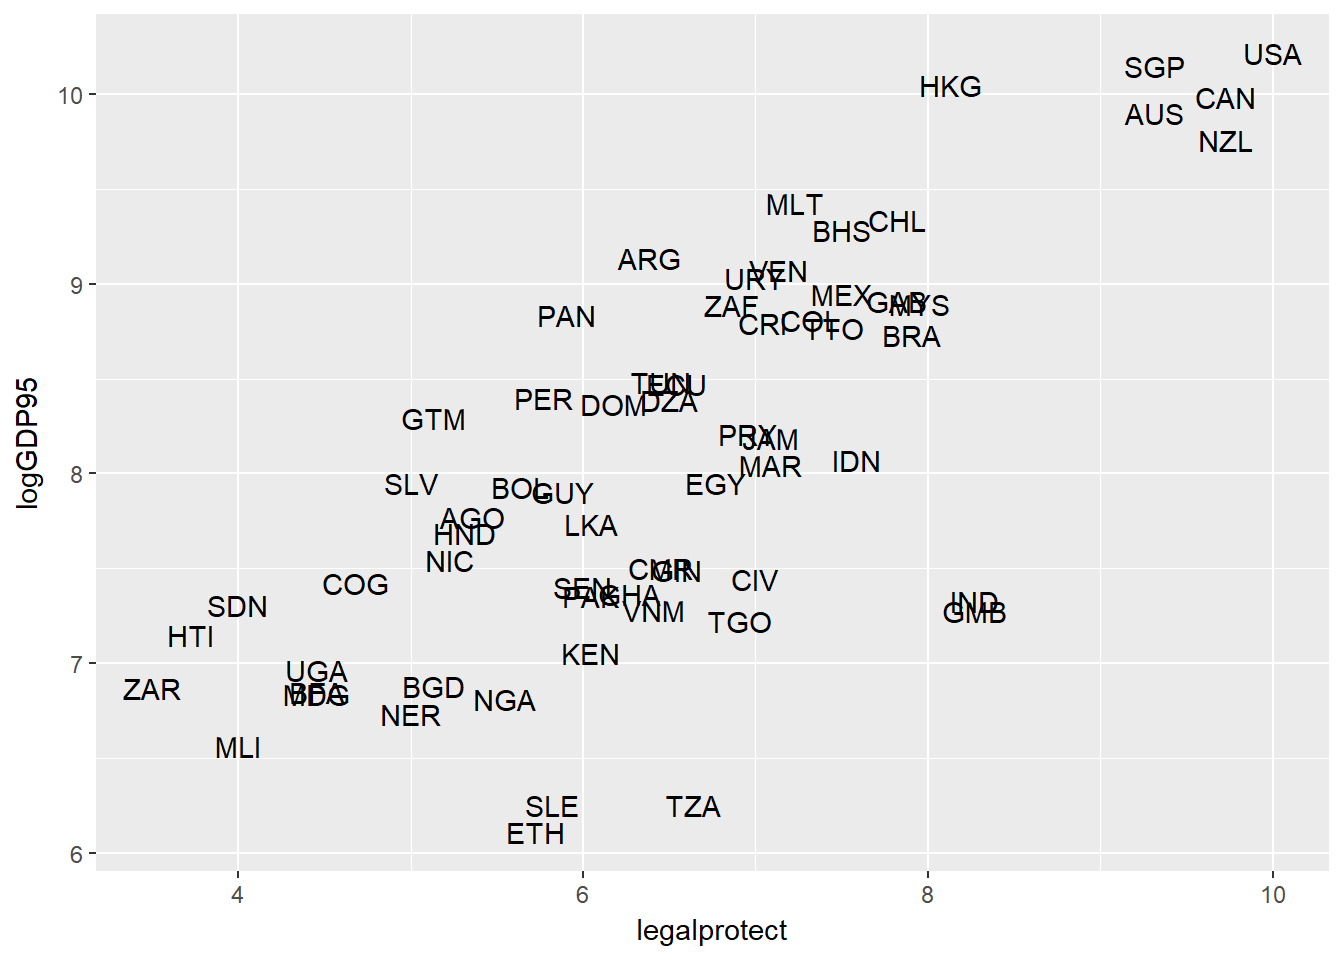
\includegraphics{module5_files/figure-beamer/unnamed-chunk-43-1.pdf}

\end{frame}

\begin{frame}[fragile]{Line graph}

A line graph uses the geometry \textbf{geom\_line()}.

\begin{Shaded}
\begin{Highlighting}[]
\KeywordTok{ggplot}\NormalTok{(col_origins, }\KeywordTok{aes}\NormalTok{(}\DataTypeTok{x=}\NormalTok{legalprotect, }
            \DataTypeTok{y =}\NormalTok{ logGDP95)) }\OperatorTok{+}\StringTok{ }\KeywordTok{geom_line}\NormalTok{()}
\end{Highlighting}
\end{Shaded}

\end{frame}

\begin{frame}{Line graph}

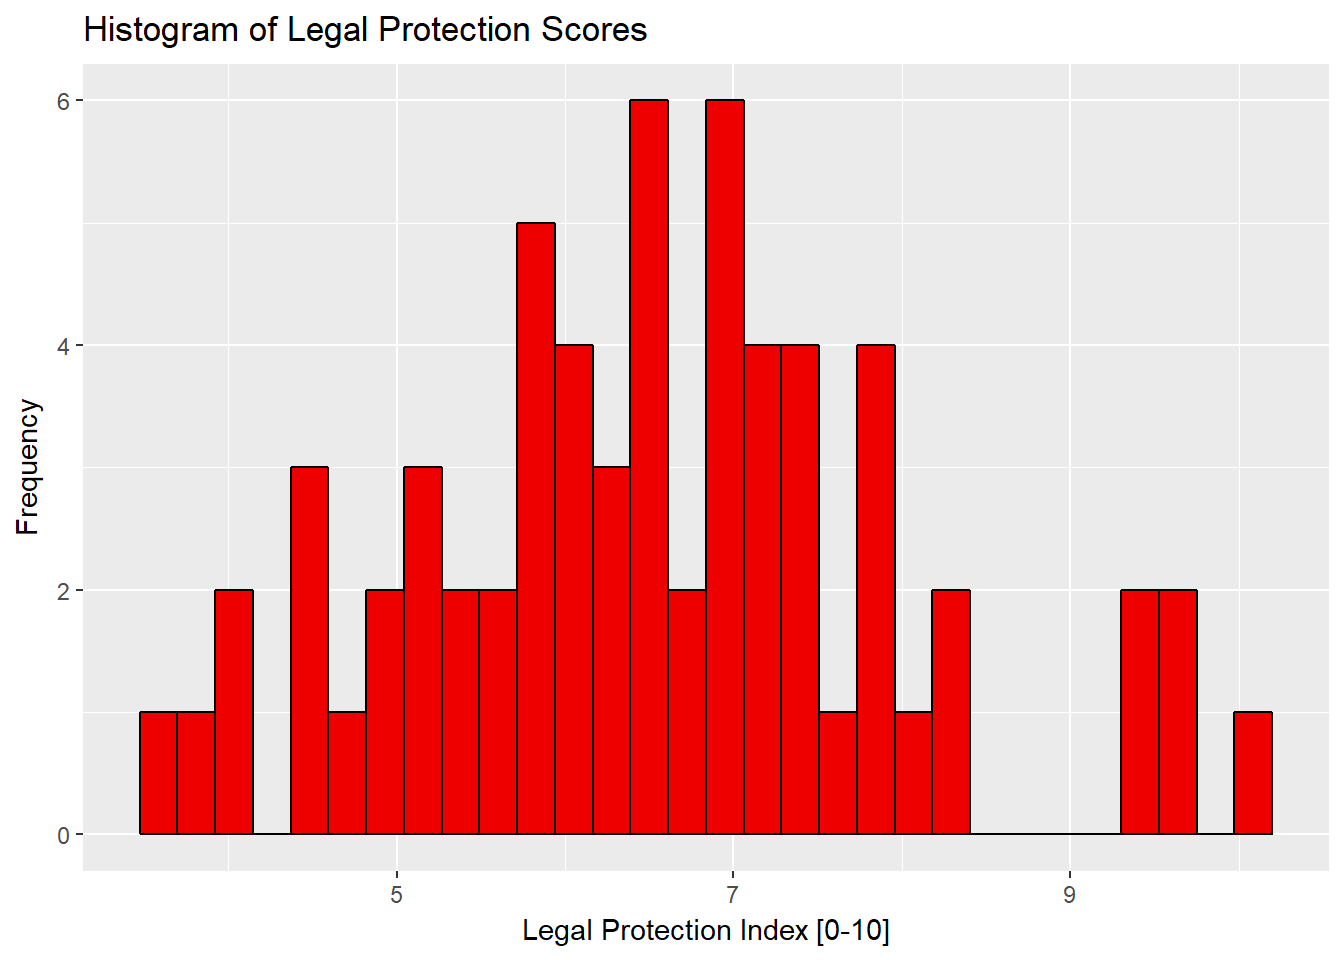
\includegraphics{module5_files/figure-beamer/unnamed-chunk-45-1.pdf}

\end{frame}

\begin{frame}[fragile]{Plotting a regression line}

A more useful line is the fitted values from the regression. Here's a
plot of that line with the points from the scatterplot for the Acemoglu
IV:

\begin{Shaded}
\begin{Highlighting}[]
\NormalTok{IV_fitted <-}\StringTok{ }\KeywordTok{tibble}\NormalTok{(col_origins}\OperatorTok{$}\NormalTok{legalprotect, }
                    \KeywordTok{fitted}\NormalTok{(col_origins_iv))}
\KeywordTok{colnames}\NormalTok{(IV_fitted) <-}\StringTok{ }\KeywordTok{c}\NormalTok{(}\StringTok{"legalprotect"}\NormalTok{, }\StringTok{"hat"}\NormalTok{)}

\KeywordTok{ggplot}\NormalTok{(col_origins, }\KeywordTok{aes}\NormalTok{(}\DataTypeTok{x=}\NormalTok{legalprotect, }
  \DataTypeTok{y =}\NormalTok{ logGDP95))  }\OperatorTok{+}\StringTok{  }\KeywordTok{geom_point}\NormalTok{(}\DataTypeTok{color=}\StringTok{"red"}\NormalTok{)  }\OperatorTok{+}\StringTok{  }
\StringTok{  }\KeywordTok{geom_line}\NormalTok{(}\DataTypeTok{data =}\NormalTok{ IV_fitted, }\KeywordTok{aes}\NormalTok{(}\DataTypeTok{x=}\NormalTok{legalprotect, }
                                  \DataTypeTok{y=}\NormalTok{hat)) }
\end{Highlighting}
\end{Shaded}

\end{frame}

\begin{frame}{Plotting a regression line}

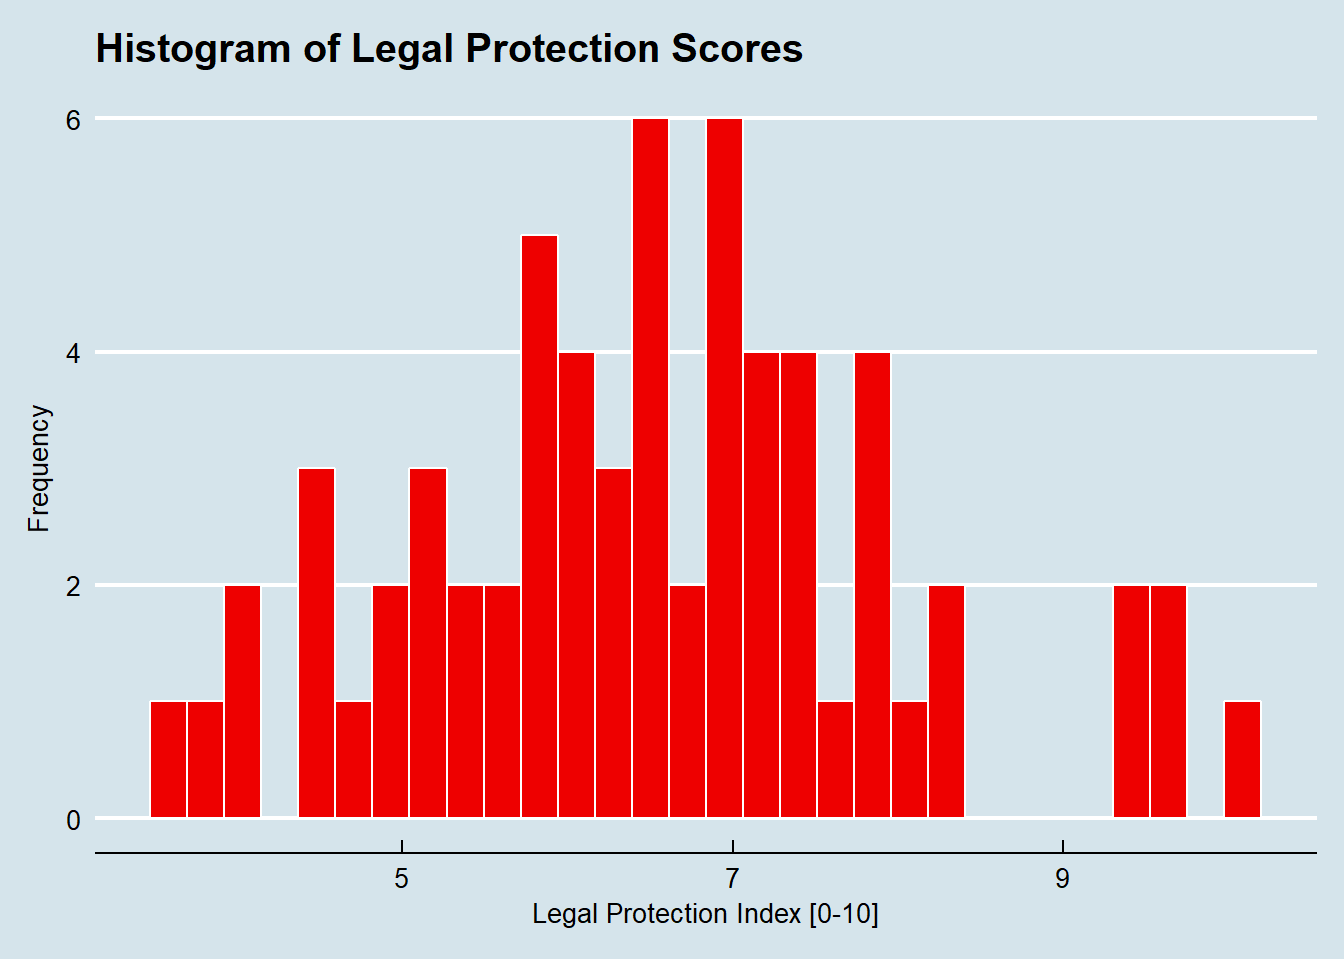
\includegraphics{module5_files/figure-beamer/unnamed-chunk-47-1.pdf}

\end{frame}

\begin{frame}[fragile]{Specifying axis and titles}

A standard task in making the graph is specifying graph titles (main and
axes), as well as potentially specifying the scale of the axes.

\begin{Shaded}
\begin{Highlighting}[]
\KeywordTok{ggplot}\NormalTok{(col_origins, }
  \KeywordTok{aes}\NormalTok{(}\DataTypeTok{x=}\NormalTok{legalprotect, }\DataTypeTok{y =}\NormalTok{ logGDP95))  }\OperatorTok{+}\StringTok{ }
\StringTok{  }\KeywordTok{geom_point}\NormalTok{(}\DataTypeTok{color=}\StringTok{"red"}\NormalTok{) }\OperatorTok{+}\StringTok{  }
\StringTok{  }\KeywordTok{geom_line}\NormalTok{(}\DataTypeTok{data =}\NormalTok{ IV_fitted, }
  \KeywordTok{aes}\NormalTok{(}\DataTypeTok{x=}\NormalTok{legalprotect, }\DataTypeTok{y=}\NormalTok{hat))  }\OperatorTok{+}\StringTok{ }
\StringTok{  }\KeywordTok{ggtitle}\NormalTok{(}\StringTok{"GDP and Legal Protection"}\NormalTok{) }\OperatorTok{+}
\StringTok{  }\KeywordTok{xlab}\NormalTok{(}\StringTok{"Legal Protection Index [0-10]"}\NormalTok{) }\OperatorTok{+}\StringTok{ }
\StringTok{  }\KeywordTok{ylab}\NormalTok{(}\StringTok{"Log of 1995 GDP"}\NormalTok{) }\OperatorTok{+}
\StringTok{  }\KeywordTok{xlim}\NormalTok{(}\DecValTok{0}\NormalTok{, }\DecValTok{10}\NormalTok{) }\OperatorTok{+}\StringTok{ }\KeywordTok{ylim}\NormalTok{(}\DecValTok{5}\NormalTok{,}\DecValTok{10}\NormalTok{)}
\end{Highlighting}
\end{Shaded}

\end{frame}

\begin{frame}{Specifying axis and titles}

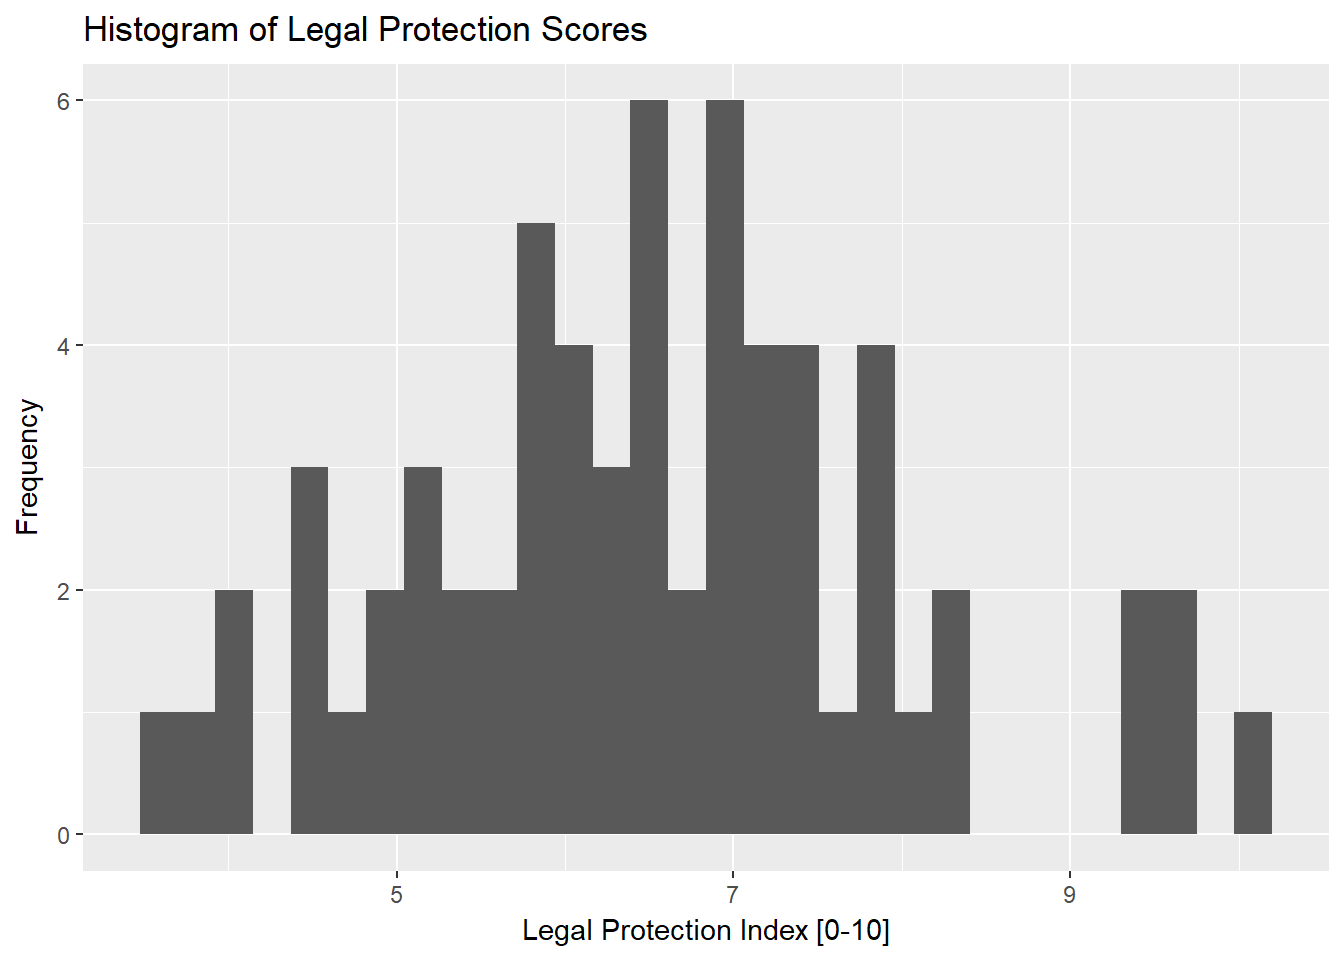
\includegraphics{module5_files/figure-beamer/unnamed-chunk-49-1.pdf}

\end{frame}

\begin{frame}[fragile]{Histogram}

The geometry point for histogram is \textbf{geom\_histogram()}.

\begin{Shaded}
\begin{Highlighting}[]
\KeywordTok{ggplot}\NormalTok{(col_origins, }\KeywordTok{aes}\NormalTok{(}\DataTypeTok{x=}\NormalTok{legalprotect)) }\OperatorTok{+}\StringTok{ }
\StringTok{  }\KeywordTok{geom_histogram}\NormalTok{() }\OperatorTok{+}\StringTok{ }
\StringTok{  }\KeywordTok{ggtitle}\NormalTok{(}\StringTok{"Histogram of Legal Protection Scores"}\NormalTok{) }\OperatorTok{+}
\StringTok{  }\KeywordTok{xlab}\NormalTok{(}\StringTok{"Legal Protection Index [0-10]"}\NormalTok{) }\OperatorTok{+}
\StringTok{  }\KeywordTok{ylab}\NormalTok{(}\StringTok{"Frequency"}\NormalTok{) }
\end{Highlighting}
\end{Shaded}

\end{frame}

\begin{frame}{Histogram}

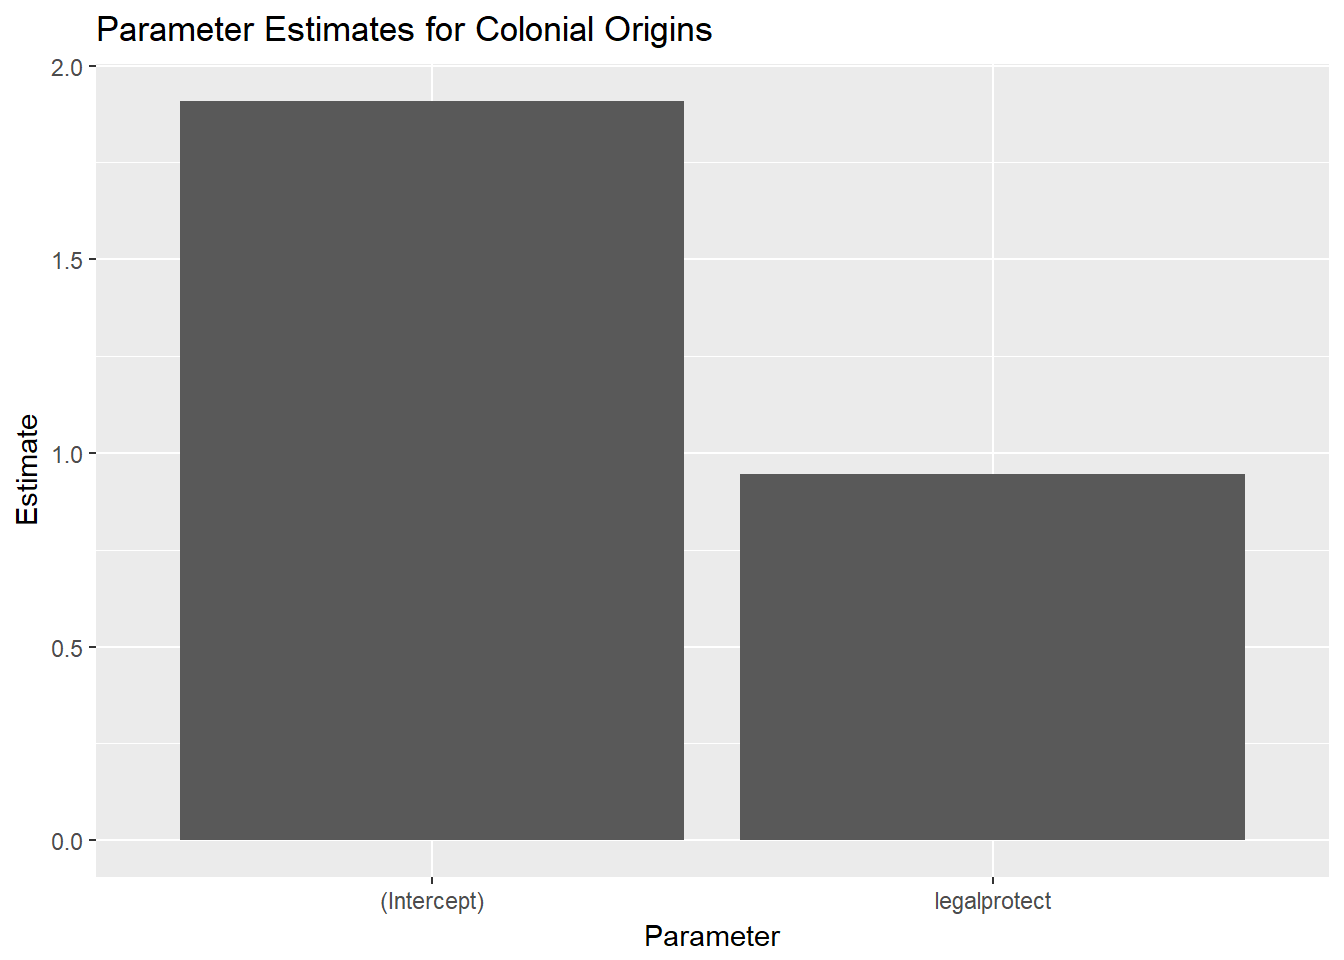
\includegraphics{module5_files/figure-beamer/unnamed-chunk-51-1.pdf}

\end{frame}

\begin{frame}[fragile]{Bar plot}

The geometry for a bar plot is \textbf{geom\_bar()}. By default, a bar
plot uses frequencies for its values, but you can use values from a
column by specifying \textbf{stat = ``identity''} inside
\textbf{geom\_bar()}.

\begin{Shaded}
\begin{Highlighting}[]
\NormalTok{coeffs_IV <-}\StringTok{ }\KeywordTok{tidy}\NormalTok{(col_origins_iv)}

\KeywordTok{ggplot}\NormalTok{(coeffs_IV, }
  \KeywordTok{aes}\NormalTok{(}\DataTypeTok{x=}\NormalTok{term, }\DataTypeTok{y=}\NormalTok{estimate)) }\OperatorTok{+}\StringTok{ }
\StringTok{  }\KeywordTok{geom_bar}\NormalTok{(}\DataTypeTok{stat =} \StringTok{"identity"}\NormalTok{) }\OperatorTok{+}\StringTok{ }
\StringTok{  }\KeywordTok{ggtitle}\NormalTok{(}\StringTok{"Parameter Estimates for Colonial Origins"}\NormalTok{) }\OperatorTok{+}
\StringTok{  }\KeywordTok{xlab}\NormalTok{(}\StringTok{"Parameter"}\NormalTok{) }\OperatorTok{+}\StringTok{ }\KeywordTok{ylab}\NormalTok{(}\StringTok{"Estimate"}\NormalTok{)}
\end{Highlighting}
\end{Shaded}

\end{frame}

\begin{frame}{Bar plot}

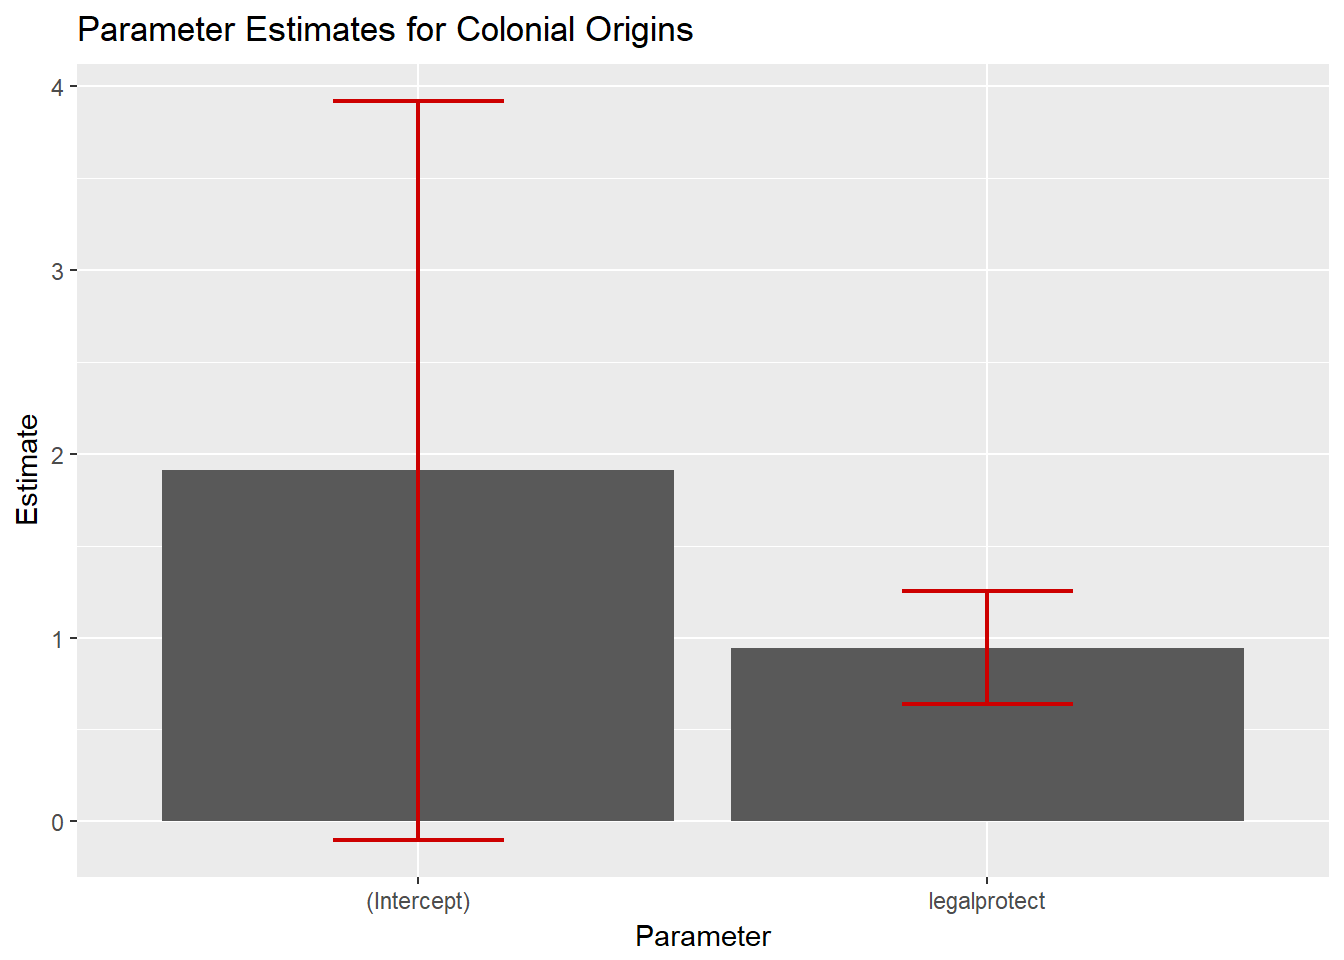
\includegraphics{module5_files/figure-beamer/unnamed-chunk-53-1.pdf}

\end{frame}

\begin{frame}[fragile]{Adding error bars}

You can easily add error bars by specifying the values for the error bar
inside of \textbf{geom\_errorbar()}.

\begin{Shaded}
\begin{Highlighting}[]
\KeywordTok{ggplot}\NormalTok{(coeffs_IV, }
  \KeywordTok{aes}\NormalTok{(}\DataTypeTok{x=}\NormalTok{term, }\DataTypeTok{y=}\NormalTok{estimate)) }\OperatorTok{+}\StringTok{ }
\StringTok{  }\KeywordTok{geom_bar}\NormalTok{(}\DataTypeTok{stat =} \StringTok{"identity"}\NormalTok{) }\OperatorTok{+}\StringTok{ }
\StringTok{  }\KeywordTok{ggtitle}\NormalTok{(}\StringTok{"Parameter Estimates for Colonial Origins"}\NormalTok{) }\OperatorTok{+}
\StringTok{  }\KeywordTok{xlab}\NormalTok{(}\StringTok{"Parameter"}\NormalTok{) }\OperatorTok{+}\StringTok{ }\KeywordTok{ylab}\NormalTok{(}\StringTok{"Estimate"}\NormalTok{) }\OperatorTok{+}
\StringTok{  }\KeywordTok{geom_errorbar}\NormalTok{(}\KeywordTok{aes}\NormalTok{(}\DataTypeTok{ymin=}\NormalTok{estimate }\OperatorTok{-}\StringTok{ }\FloatTok{1.96} \OperatorTok{*}\StringTok{ }\NormalTok{std.error, }
                    \DataTypeTok{ymax=}\NormalTok{estimate }\OperatorTok{+}\StringTok{ }\FloatTok{1.96} \OperatorTok{*}\StringTok{ }\NormalTok{std.error), }
                    \DataTypeTok{size=}\NormalTok{.}\DecValTok{75}\NormalTok{, }\DataTypeTok{width=}\NormalTok{.}\DecValTok{3}\NormalTok{, }\DataTypeTok{color=}\StringTok{"red3"}\NormalTok{)}
\end{Highlighting}
\end{Shaded}

\end{frame}

\begin{frame}{Adding error bars}

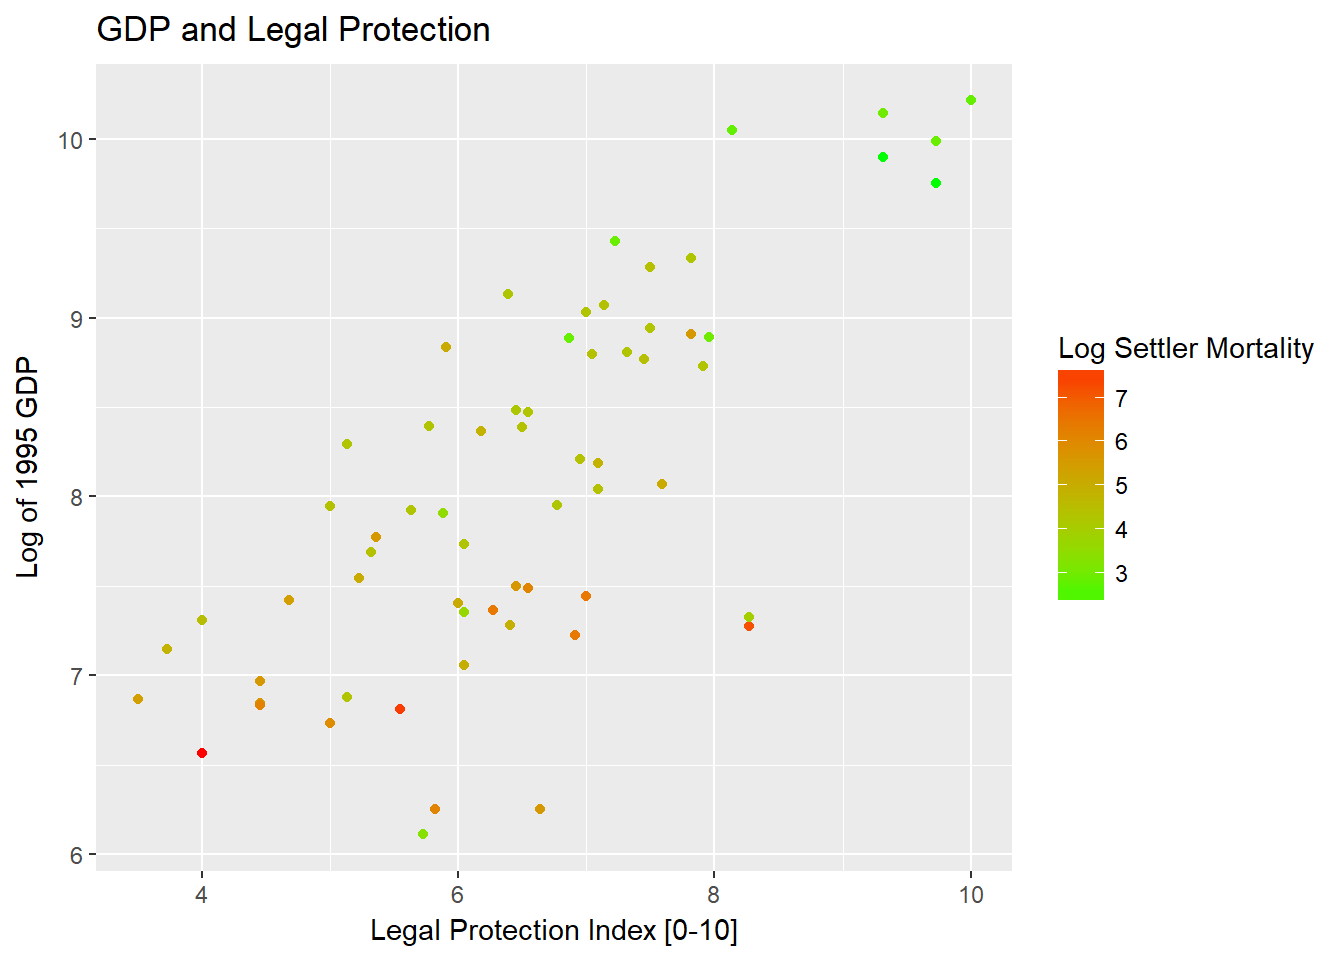
\includegraphics{module5_files/figure-beamer/unnamed-chunk-55-1.pdf}

\end{frame}

\begin{frame}[fragile]{Adding colors}

You can easily add color to graph points as well. There are a lot of
aesthetic options to do that --- here I demonstrate adding a color
\emph{scale} to the graph.

\begin{Shaded}
\begin{Highlighting}[]
\KeywordTok{ggplot}\NormalTok{(col_origins, }\KeywordTok{aes}\NormalTok{(}\DataTypeTok{x=}\NormalTok{legalprotect, }
  \DataTypeTok{y =}\NormalTok{ logGDP95 , }\DataTypeTok{col=}\NormalTok{ log.settler.mort)) }\OperatorTok{+}
\StringTok{  }\KeywordTok{geom_point}\NormalTok{() }\OperatorTok{+}\StringTok{ }
\StringTok{  }\KeywordTok{ggtitle}\NormalTok{(}\StringTok{"GDP and Legal Protection"}\NormalTok{) }\OperatorTok{+}
\StringTok{  }\KeywordTok{xlab}\NormalTok{(}\StringTok{"Legal Protection Index [0-10]"}\NormalTok{) }\OperatorTok{+}\StringTok{ }
\StringTok{  }\KeywordTok{ylab}\NormalTok{(}\StringTok{"Log of 1995 GDP"}\NormalTok{) }\OperatorTok{+}\StringTok{ }
\StringTok{  }\KeywordTok{scale_color_gradient}\NormalTok{(}\DataTypeTok{low=}\StringTok{"green"}\NormalTok{,}\DataTypeTok{high=}\StringTok{"red3"}\NormalTok{, }
                       \DataTypeTok{name=}\StringTok{"Log Settler Mortality"}\NormalTok{)}
\end{Highlighting}
\end{Shaded}

\end{frame}

\begin{frame}{Adding colors}

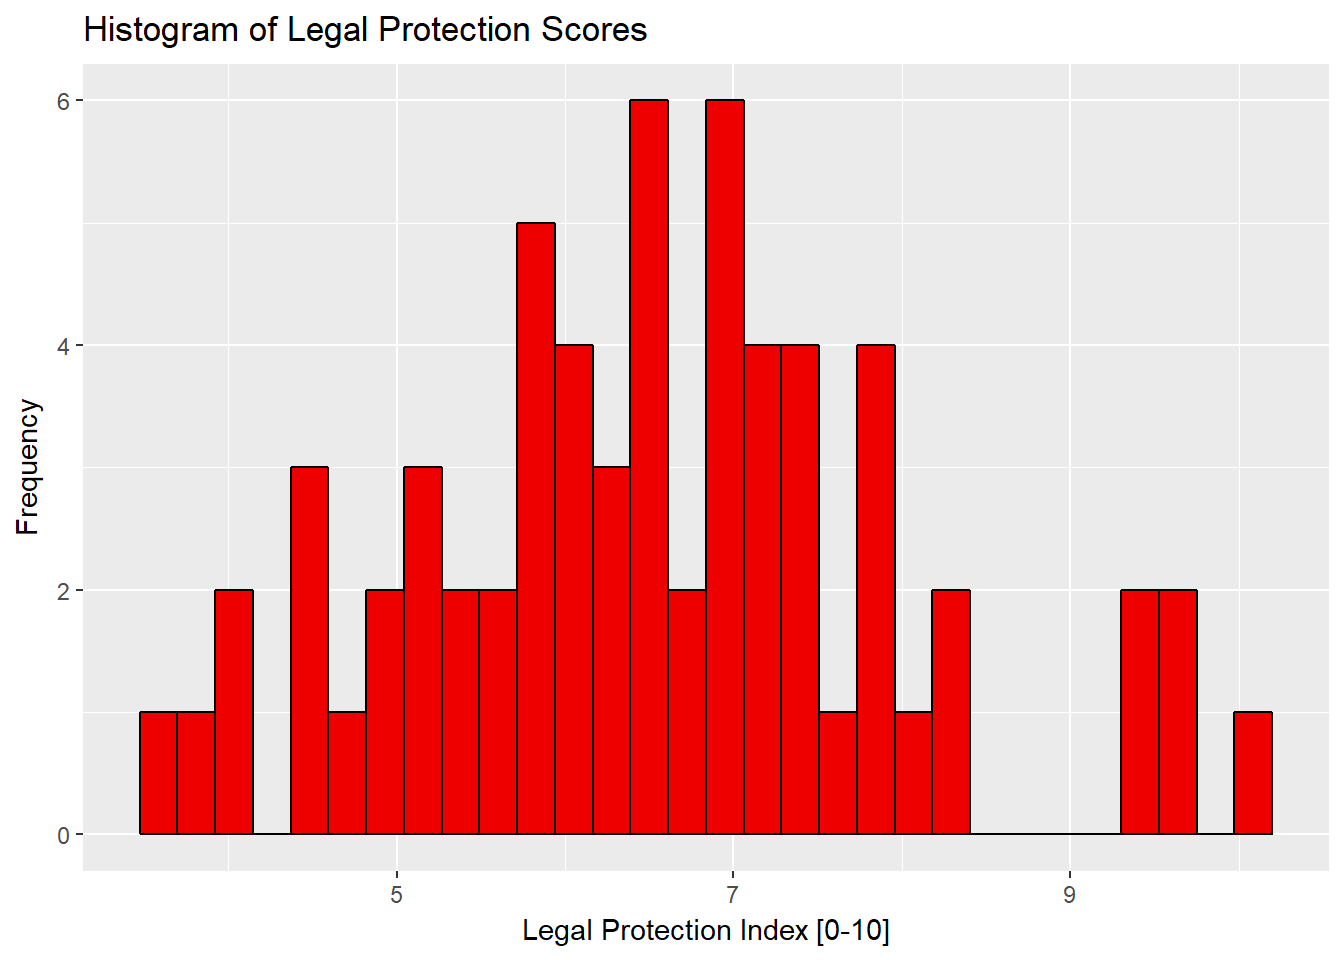
\includegraphics{module5_files/figure-beamer/unnamed-chunk-57-1.pdf}

\end{frame}

\begin{frame}[fragile]{Adding colors: example 2}

\begin{Shaded}
\begin{Highlighting}[]
\KeywordTok{ggplot}\NormalTok{(col_origins, }\KeywordTok{aes}\NormalTok{(}\DataTypeTok{x=}\NormalTok{legalprotect)) }\OperatorTok{+}\StringTok{ }
\StringTok{  }\KeywordTok{geom_histogram}\NormalTok{(}\DataTypeTok{col=}\StringTok{"black"}\NormalTok{, }\DataTypeTok{fill=}\StringTok{"red2"}\NormalTok{) }\OperatorTok{+}\StringTok{ }
\StringTok{  }\KeywordTok{ggtitle}\NormalTok{(}\StringTok{"Histogram of Legal Protection Scores"}\NormalTok{) }\OperatorTok{+}
\StringTok{  }\KeywordTok{xlab}\NormalTok{(}\StringTok{"Legal Protection Index [0-10]"}\NormalTok{) }\OperatorTok{+}
\StringTok{  }\KeywordTok{ylab}\NormalTok{(}\StringTok{"Frequency"}\NormalTok{) }
\end{Highlighting}
\end{Shaded}

\end{frame}

\begin{frame}{Adding colors: example 2}

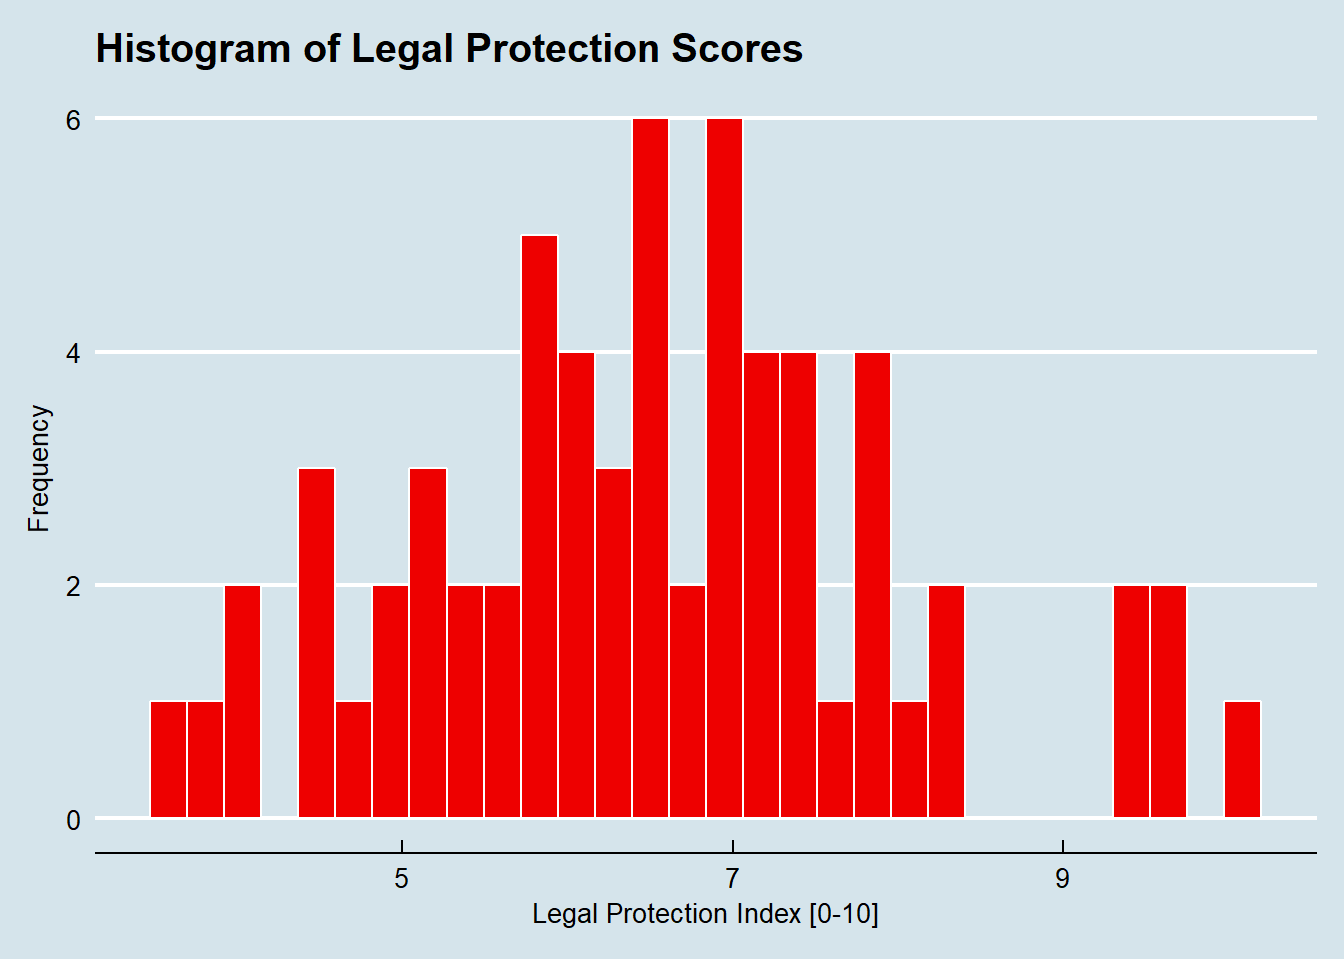
\includegraphics{module5_files/figure-beamer/unnamed-chunk-59-1.pdf}

\end{frame}

\begin{frame}[fragile]{Adding themes}

Another option to affect the appearance of the graph is to use
\textbf{themes}, which affect a number of general aspects concerning how
graphs are displayed.

\begin{itemize}
\tightlist
\item
  Some default themes come installed with ggplot2/tidyverse, but some of
  the best in my opinion come from the package
  \href{https://github.com/jrnold/ggthemes}{ggthemes}.
\end{itemize}

\begin{Shaded}
\begin{Highlighting}[]
\KeywordTok{library}\NormalTok{(ggthemes)}
\end{Highlighting}
\end{Shaded}

\end{frame}

\begin{frame}[fragile]{Adding themes}

\begin{itemize}
\tightlist
\item
  To apply a theme, just add \textbf{+ themename()} to your ggplot
  graphic.
\end{itemize}

\begin{Shaded}
\begin{Highlighting}[]
\KeywordTok{ggplot}\NormalTok{(col_origins, }\KeywordTok{aes}\NormalTok{(}\DataTypeTok{x=}\NormalTok{legalprotect)) }\OperatorTok{+}\StringTok{ }
\StringTok{  }\KeywordTok{geom_histogram}\NormalTok{(}\DataTypeTok{col=}\StringTok{"white"}\NormalTok{, }\DataTypeTok{fill=}\StringTok{"red2"}\NormalTok{) }\OperatorTok{+}\StringTok{ }
\StringTok{  }\KeywordTok{ggtitle}\NormalTok{(}\StringTok{"Histogram of Legal Protection Scores"}\NormalTok{) }\OperatorTok{+}
\StringTok{  }\KeywordTok{xlab}\NormalTok{(}\StringTok{"Legal Protection Index [0-10]"}\NormalTok{) }\OperatorTok{+}
\StringTok{  }\KeywordTok{ylab}\NormalTok{(}\StringTok{"Frequency"}\NormalTok{) }\OperatorTok{+}\StringTok{ }
\StringTok{  }\KeywordTok{theme_economist}\NormalTok{()}
\end{Highlighting}
\end{Shaded}

\end{frame}

\begin{frame}{Adding themes}

\includegraphics{module5_files/figure-beamer/unnamed-chunk-62-1.pdf}

\end{frame}

\begin{frame}{More with ggplot2}

This has been just a small overview of things you can do with ggplot2.
To learn more about it, here are some useful references:

\href{http://ggplot2.tidyverse.org/}{\textbf{The ggplot2 website:}}

\begin{itemize}
\tightlist
\item
  Very informative although if you don't know what you're looking for,
  you can be a bit inundated with information.
\end{itemize}

\href{http://www.sthda.com/english/wiki/ggplot2-essentials}{\textbf{STHDA
Guide to ggplot2:}}

\begin{itemize}
\tightlist
\item
  A bit less detailed, but a good general guide to ggplot2 that is still
  pretty thorough.
\end{itemize}

\textbf{\href{https://github.com/rstudio/cheatsheets/raw/master/data-visualization-2.1.pdf}{RStudio's
ggplot2 cheat sheet}:}

\begin{itemize}
\tightlist
\item
  As with all the cheat sheets, very concise but a great short reference
  to main options in the package.
\end{itemize}

\end{frame}

\end{document}
